\section{Calculo de secuentes.}


Para traducir el uso de modelos de Kripke a secuentes, es necesario saber como codificar los diversos mundos. Esto se puede hacer mediante el uso de etiquetas en la los secuentes de la lógica clásica. No solo eso, esta codificación tiene la ventaja de permitir una separación parcial entre las reglas lógicas del sistema y propiedades sobre la relación binaria del modelo de Kripke. Dicha separación parcial permite utilizar estructuras complejas sobre la relación manteniendo admisibles las reglas estructurales de weakening y cut.

Dicho esto, nuestros contextos son multiconjuntos cuyos elementos son formulas modales etiquetadas por su mundo $w:A$ para indicar que $w \V A$ y átomos relacionales $wRo$.


Las reglas para el calculo de secuentes de \K forman el sistema llamado G3Kse muestran a continuación para $\Gamma$ y $\Delta$ contextos.


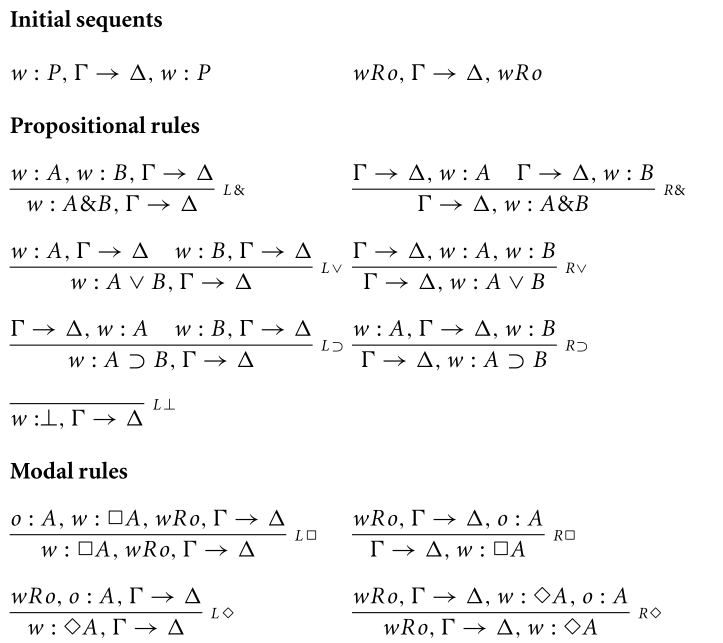
\includegraphics[width=\textwidth]{reglas} 

En los secuentes iniciales $P$ es una formula atómica arbitraria. 
En $R\necesidad$ y $L\posibilidad$, la $o$ es una variable fresca.

Ahora se puede apreciar la separación mencionada al observar que la regla de secuente inicial para $R$ es la única que permite el uso de los átomos relacionales en el lado derecho del $\derives$.


Debemos traducir los axiomas \eqref{eqn:4axiom} y \eqref{eqn:taxiom} a este calculo de secuentes. 

El primer caso es simple pues la reflexividad es fácil de expresar.

\begin{align*}
  \tree{Ref}{wRw, \Gamma \derives \Delta}{\Gamma \derives \Delta} \\
  \tree{Trans}{wRr, wRo, oRr \Gamma \derives \Delta}{wRo, oRr, \Gamma \derives \Delta}
\end{align*}

El caso de la transitividad requiere un poco mas de atención pues, la regla esquematica para la forma de traducir axiomas a reglas de secuentes indicaria el uso de una sola $wRr$ en el lado izquierdo del antecedente si se usara de forma ciega.


Con estas dos reglas tenemos el sistema con el que vamos a trabajar G3S4. Por conveniencia continuaremos mencionándolo como S4 salvo que indiquemos lo contrario.

